\section{Datenverarbeitung}
	
	In diesem Kapitel wird näher auf den Programmcode des vorliegenden Forschungsprojektes eingegangen und erklärt, was genau in der Datensammlung und Datenverarbeitung 
	gemacht wurde. 
	Als Erstes hat das Forscherteam die Daten wie in Punkt 2.1.1 GetOldTweets3 beschrieben, mit der Bibliothek gescrapped und als csv-Datei abgespeichert. Wie das Sracpping 
	in der Bibliothek genau funktioniert, ist ebenfalls unter dem Punkt 2.1.1. GetOldTweets3 beschrieben. Um die gespeicherten Tweets für das Mapreduce vor zu verarbeiten, 
	nutzen das Team die zur Verfügung stehenden Bibliotheken NLTK und cleantext.
	
	
	\begin{figure}[ht]
		\centering
		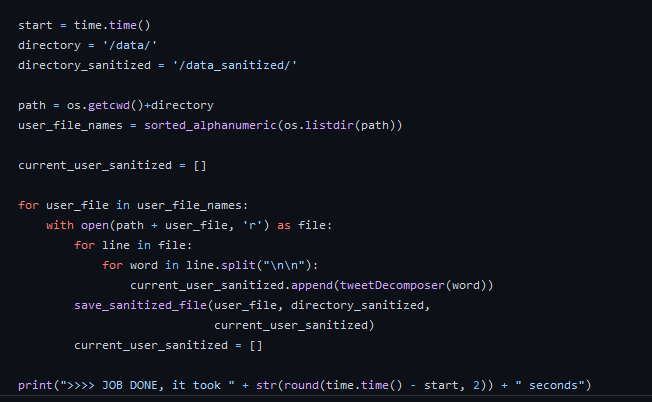
\includegraphics[width=0.9\textwidth]{images/Kapitel2/Code_Datensanierung_1}
		\caption{\label{fig:DataSan}Sanierungs-For-Schleife der Daten}
	\end{figure}
	
	Die Variable "directory" und "directory\_ Sanitized" geben den Path an, in welchen Ordner die Daten gespeichert werden sollen. Mit der Bibliothek os von Python kann man 
	zum Beispiel über "os.listdir(Path)" alle Dateinamen innerhalb dieses Ordners einlesen lassen. 
	Über die Variable user\_ file\_ names bekommt man eine alphanumerisch sortierte Liste der Usernamen der Politiker zurück, welche dann über eine FOR-Schleife durchgegangen 
	werden, da der Name der CSV-Dateien mit folgenden Muster den Usernames entspricht, "Name\_ D" oder "Name\_ R". D steht für demokratisch und R für 
	republikanisch. In dieser Datensanierungsschleife wird die Funktion tweetDecomposer verwendet. Diese Funktion übernimmt in der vorliegenden Datensanierung die 
	Hauptaufgabe.\\
	
%	\begin{figure}[ht]
%		\centering
%		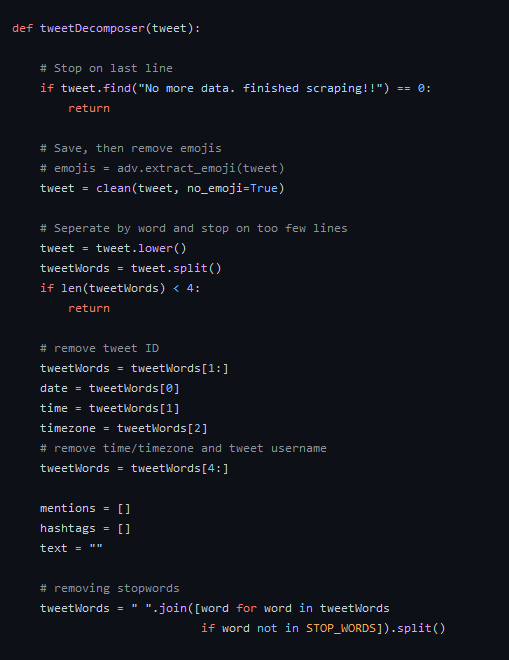
\includegraphics[width=0.9\textwidth]{images/Kapitel2/Code_Datensanierung_2}
%		\caption{\label{fig:DataSanF1}Ausschnitt eins der Sanierungsfunktion der Daten}
%	\end{figure}

	Mit dem Bibliothek cleantext wurden die Emojis aus dem Text entfernt, wie man in Abbildung ~\ref{fig:DataSanF1} in den ersten Zeilen der Funktion sehen kann.
	Dann werden alle Worte innerhalb eines Tweets kleingeschrieben und aufgetrennt, damit dann die ID, die Zeitzone und der Username aus dem Tweet entfernt werden kann. Mit 
	NLTK werden dann die Stoppworte durch ein join aus den Tweets entfernt, so das man zu den letzten Datensanierungsschritten kommen kann.\\
	 
%	\begin{figure}[ht]
%		\centering
%		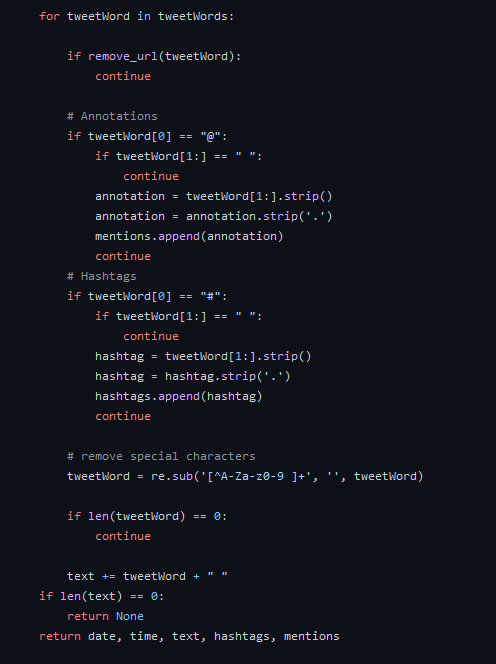
\includegraphics[width=0.9\textwidth]{images/Kapitel2/Code_Datensanierung_3}
%		\caption{\label{fig:DataSanF1}Ausschnitt eins der Sanierungsfunktion der Daten}
%	\end{figure}
	
	Da die Annotationen und Hashtags gespeichert werden sollen, wurde, wie in Abbildung ~\ref{fig:DataSanF2} zu sehen ist,  eine extra FOR-Schleife dafür verwendet. Die FOR-
	Schleife läuft über den gesamten Input des Tweets, dazu zählt Datum, Zeit, Username, Hashtags, Emoji usw. Als Erstes wird überprüft, ob es sich um eine URL handelt oder 
	nicht. Tritt der Fall ein, dass es eine URL ist, wird diese einfach übersprungen und nicht mit abgespeichert. Die Annotation können durch eine "@" erkannt werden, während 
	die Hashtags mit einem "\# " erkannt werden. Beide Erkennungsmaker werden nicht mit abgespeichert. Der restliche Inhalt des Hashtags und der Annotationen werden in einer 
	Liste gespeichert. Als Letztes haben wir alles Spezielle Charakter wie Punkte, Kommas usw. entfernt aus den tweetword. Die Funktion gibt dann alle interessanten Daten wie 
	Datum, Zeit, den Textinhalt des Tweets, die Hashtags und die mentions, für die Analyse zurück. Zum Schluss werden diese Daten in einer CSV-Datei gespeichert Ordner data\_ 
	sanitized. Als nächster Schritt folgt die Hautanalyse unseres Projektes in 2.3
	
